\section{Case Study}
% overpic environment: for adjustments use \begin{overpic}[grid,tics=10]...
\begin{frame}[fragile]
  \frametitle{Case Study}
  A language to specify a GUI to edit entities
  
  \begin{columns}[T]
        \column{.4\textwidth}
%        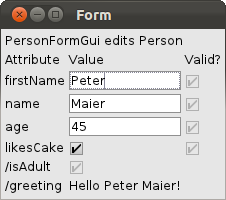
\includegraphics[scale=0.6]{img/form-valid.png}
        \begin{overpic}[scale=0.6]%
          {img/form-valid.png}
          \only<2>{
          \put(55,-40){\includegraphics[scale=0.6]%
          {img/form-invalid.png}}}
        \end{overpic}
        \column{.6\textwidth}
\note{          \begin{itemize}
            \item Entities
            \begin{itemize}
              \item primitive attributes
              \item derived attributes
            \end{itemize}
            \only<1>{
            \item Forms
            \begin{itemize}
              \item textboxes
              \item checkboxes
              \item validation clauses
            \end{itemize}
            }
          \end{itemize}
}          
  \end{columns}
\note{BTW, entities support inheritance \\

}
\end{frame}

\begin{frame}
	\frametitle{Case Study} % for adjustments use overpic[grid,tics=10]  
	\begin{overpic}[scale=0.5]%
       {img/guidsl.png}
       \visible<2->{
        \put(-2.5,-3){\includegraphics[scale=0.5]%
		{img/guidsl-errors$1.png}}}
       \begin{tikzpicture}[overlay]
		\draw<2-> [thick,color=red](3.0cm,0.75cm) ellipse (.65cm and .22cm);
       \end{tikzpicture}
%        \visible<3->{
%        \put(50,22){
%          \begin{minipage}{0.50\textwidth}
%           Running example: Plus operator
%          \end{minipage}}}
     \end{overpic}
%        \begin{tikzpicture}[overlay]
% 		\draw<3-> [thick,color=red](4.4cm,3.85cm) ellipse (2.15cm and .3cm);
%        \end{tikzpicture}
\end{frame}